\documentclass[twocolumn]{article}
\usepackage[utf8]{inputenc}
\usepackage[english]{babel}
\usepackage{lipsum}
\usepackage{multicol}
\usepackage{abstract} % Allows abstract customization
\usepackage{footnote}
\usepackage{listings}
\usepackage{url}
\usepackage{dblfnote}
\usepackage{graphicx}
\usepackage{algorithmicx}
\usepackage[noend]{algpseudocode}
\setlength{\columnsep}{1cm}
 

\begin{document}

\twocolumn[\begin{@twocolumnfalse}
  \centerline{\Large\bfseries Optimizing Small Scale Combat With Neural Networks}
  \vspace{3ex}
  \centerline{Peixian Wang}
  \centerline{May 3, 2016}
  \vspace{3ex}
\end{@twocolumnfalse}]

\begin{abstract}
A major challenge in real-time strategy games is individual unit control, where the player must issue separate orders and deploy units in different places in order to maximize the effectiveness of a single unit. Starcraft: Brood War (henceforth referred to as Starcraft), a real-time strategy game released in 1998 by Blizzard Entertainment, provides a ripe environment for optimization within combat deployment. We present a backpropagation neural network design that hooks into the Alpha-Beta combat algorithm, which then allows an AI to consistently position units before combat in a manner to beat the build-in computer AI. 
\end{abstract}

\section{Introduction}
Micro-management, or the management of units on an individual scale, is an extremely integral part of modern real-time strategy (RTS) games today. Players are required to move units in order to gather resources, construct buildings, or engage in combat. Within combat alone, effective players must decide: 1. which units to engage with, 2. proper battlefield to engage on, and 3. where the engaging units should be placed. Oftentimes, this level of decision making has happened on the scale of seconds for human players, where quick decision making is oftentimes rewarded with a succesful engagement. Due to the fast-paced nature of combat micro-management, decisions are oftentimes complex despite only having a small number of units. 

Modern RTS's provide a limited amount of assistance within micro-mangement, commands can be issued en masse to a group of units. However, effective management of units on an individual scale oftentimes lead to a more favorable outcome, such as the technique called Scourge Cloning\footnote{\tiny{\url{http://wiki.teamliquid.net/starcraft/Scourge_Cloning}}}. While players are able to devise complex techniques in order to work around the limitations of Starcraft itself and selectively issue batch commands when necessary, AI playing Starcraft do not have access to the same nuances and quick decision making a player does. Consider the following scenario: a player has a heterogeneous distribution of units, with both units that can only attack within a very small melee range (melee units) and units that attack from a distance (ranged units). A good player would know to place melee units in front of the ranged units in order to maximize combat effectiveness when moving the group, as the ranged units can still fire upon the enemy when the melee units are attacking the enemy, but the melee units would be blocked behind the ranged units if unit positions were switched around. To an AI, however, this distribution of units looks homogeneous, there is no easy way for the AI to realize that ranged units would be more effective if placed at a distance behind the melee units. 

This combat-oriented domain of micro-management is extremely well-suited for the applications of neural networks, as neural networks can learn the proper positioning of units based upon repeated trials and a large corpus of training data. In this paper we present an application of a neural network trained through backpropagation, over the course of 3000 games an AI properly learns the correct positioning of a small melee unit called the Zergling. In section 2 we discuss some background on Starcraft and SparCraft, a combat simulation program. In section 3 we discuss the technology stack used to enable this neural network and the AI itself, along with introducing our AI called Ultralisk. Section 4 recounts the technological approach to solving the problem, including the topology of the neural network, obtaining training data through SparCraft, and feeding the data into the Alpha-Beta combat algorithm. Section 5 and 6 detail the results of the simulation and experiment trials, along with concluding and discussing the interpretations of the results. 

\section{Background}
\begin{figure}
	\begin{center}
		\includegraphics[width=4cm]{zergling.png}
	\end{center}
	\caption{\textit{A Zergling, the basic Zerg infantry unit. }}
	\label{fig:zergling}
\end{figure}
\begin{figure}
	\begin{center}
		\includegraphics[width=4cm]{zealot.png}
	\end{center}
	\caption{\textit{A Zealot, the basic Protoss infantry unit.}}
	\label{fig:zealot}
\end{figure}
\begin{figure}
	\begin{center}
		\includegraphics[width=4cm]{marine.png}
	\end{center}
	\caption{\textit{A Marine, the basic Terran infantry unit.}}
	\label{fig:marine}
\end{figure}
\subsection{Starcraft}
Starcraft is an extremely complex game that has captured an entire country, becoming the first major e-sport. At a high level, Starcraft consists of 3 stages:

\begin{enumerate}
  \item Use units to gather resources (called \textit{Minerals} and \textit{Vespene Gas}).
  \item Spend resources to construct buildings, which enable gathering more resources and constructing more powerful units (called \textit{expanding} and \textit{moving up the tech tree} respectively). 
  \item Use the accumulated units to engage the enemy units, with the eventual goal of destroying all of the enemy buildings and units. 
\end{enumerate}

Starcraft is a robust game, consisting of 3 races (called the \textit{Zerg}, the \textit{Protoss}, and the \textit{Terran}), each with their own unique buildings and units. In order to meet the time constraints, we focused the three basic infantry units in particular, each for a single race: 

\begin{enumerate}
  \item Zerg - Zergling (Figure \ref{fig:zergling}) - A small, melee-ranged, fast-moving unit with 35 health points (HP)
  \item Protoss - Zealot (Figure \ref{fig:zealot}) - A medium-sized, melee-ranged, moderate-moving unit with 160 HP
  \item Terran - Marine (Figure \ref{fig:marine}) - A small, ranged, moderate-moving unit with 50 HP
\end{enumerate}

As these 3 units form the backbone of any army, we felt it was necessary to train the neural network on all 3 units. Due to time constraints, the AI we built (henceforth referred to as Ultralisk) is only able to utilize Zerglings, but can play against any race. 

\begin{figure}[ht]
	\begin{center}
		\includegraphics[width=8cm]{sparcraft.png}
	\end{center}
	\caption{\textit{A SparCraft simulation of 50 Zerglings vs 50 Zerglings. }}
	\label{fig:sparcraft}
\end{figure}

\subsection{SparCraft}
SparCraft\footnote{\tiny{\url{https://github.com/davechurchill/ualbertabot/wiki/SparCraft-Home}}} (shown in figure \ref{fig:sparcraft})is an open source abstract combat simulator written by David Churchill, from the University of Alberta for combat simulations. While it is \textit{not} a Starcraft combat engine, rather, it is able to accurately model unit size, damage, and movement. Because it is able to simulate combat extremely quickly, it was chosen to generate a corpus of training data for the neural network. 

SparCraft runs on a chosen map size, the map size chosen for this experiment was $1280$ x $740$, which creates a grid of 1280 by 740 cells. Each unit occupies 1 grid area, and each unit has a speed per frame. The Zergling for example, can move 1.5 grid points in any direction (it can move across its own cell and half of the next cell), while both the Zealot and the Marine can only move 1 grid point. The Marine, however, can begin attacking a target 4 cells away, while both the Zergling and Zealot can only attack units in the cell directly next to them. 

\section{Technology Stack}
\begin{figure}[ht]
	\begin{center}
		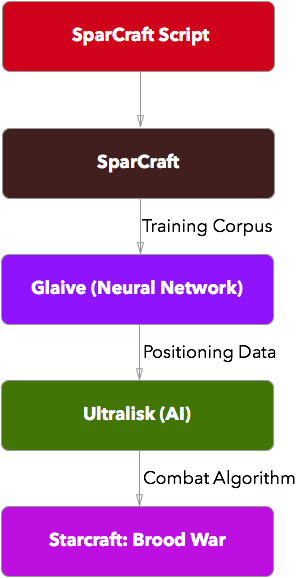
\includegraphics[width=4cm]{techStack.png}
	\end{center}
	\caption{\textit{Ultralisk technology stack, scripts run SparCraft combat simulations to generate a training corpus, which is then fed into Glaive. Glaive generates positioning data, which is then fed into Ultralisk, which then is carried out in the Starcraft game itself. }}
	\label{fig:techStack}
\end{figure}

\subsection{Overview}
Ultralisk\footnote{\tiny{\url{https://github.com/peixian/Ultralisk}}} is composed of two parts: 1. Glaive, the neural network that reads training data, and 2. the Ultralisk AI itself. The technology stack is show in figure \ref{fig:techStack}. By scripting SparCraft to generate hundreds of combat scenarios and then filtering those combat scenarios for preferred results, a large training corpus is generated. This training data is then fed into Glaive, which uses backpropagation to train itself. After convergence, the neural network generates data for Ultralisk to follow within its combat algorithm, which then enables Ultralisk to assign optimal unit positions. 

\subsection{SparCraft Scripts}
\begin{figure}[ht]
	\begin{center}
		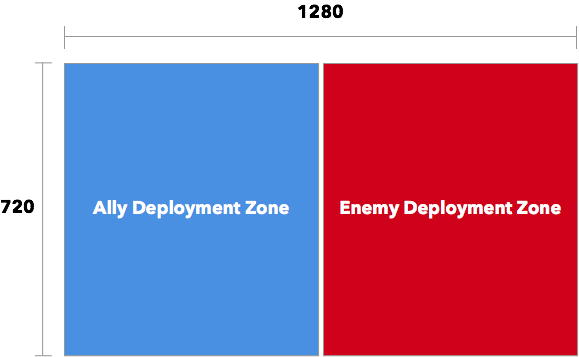
\includegraphics[width=8cm]{deploymentZones.png}
	\end{center}
	\caption{\textit{Zones where the units can be deployed, left half is where the script can deploy ally units, right half is where the enemy can deploy its units. }}
	\label{fig:zones}
\end{figure}
The SparCraft scripts are meant to generate a large training corpus for Glaive to train itself on. In order to accomplish this, the scripts create two zones, shown in figure \ref{fig:zones}. The left, blue zone is where the ally can deploy its 3 Zerglings, while the right, red zone is where the enemy can deploy its choice of units between 3 Zerglings, 2 Zealots, or 3 Marines (Zealots have a very high HP value and are considered stronger than the other infantry units in a one-on-one combat scenario, thus explaining the smaller amount of Zealots). The script then runs through 1000 scenarios, randomly generating locations for both the enemy and the ally, and then sets these locations into SparCraft to simulate the combat. The reasoning for equal deployment was due to the symmetrical nature of real Starcraft maps, meaning that the combat simulation must be symmetrical as well, leading to a division of a flat, rectangular map into two portions. If the ally is victorious after the simulation is complete, the script saves both the enemy positions and ally positions into the corpus to be trained on by Glaive later, with the enemy positions being the input (domain) and the ally positions being the target (range).

\subsection{Glaive}
\begin{figure}
	\begin{center}
		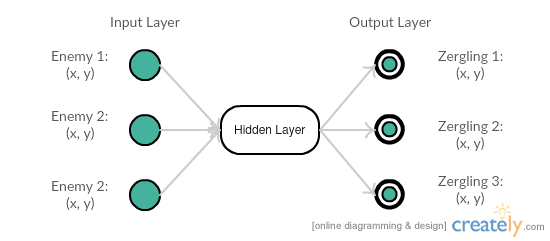
\includegraphics[width=8cm]{../plots/nnLayout.png}
	\end{center}
	\caption{\textit{Glaive has 3 input nodes and 3 output nodes. It reads the tuples of the enemy positions (x, y) for up to 3 enemies, and then generates 3 tuples with the locations of where the ally units should be placed. }}
	\label{fig:glaive}
\end{figure}
Glaive (figure \ref{fig:glaive}) is a neural network with 3 input nodes and 3 output nodes. While we used 100 hidden nodes in 1 hidden layer along with bias nodes, Glaive itself can take any arbitrary amount of hidden nodes. Each input node takes in a tuple of values, $(x_{enemy, i}, y_{enemy, i})$ for each enemy unit $i$, and then generates 3 tuples at the output nodes $(x_{ally, j}, y_{ally, j})$ for each ally unit $j$. Each tuple, before being processed by Glaive, is first normalized to between $-1$ and $1$, in order to facilitate the outcome of the neural network. After Glaive is trained to convergence, the weights within are saved to be passed into Ultralisk. 

\subsection{Ultralisk AI}
The Ultralisk AI is a C++ AI forked from UAlbertaBot\footnote{\tiny{\url{https://github.com/davechurchill/ualbertabot}}}, which is a bot utilizing BWAPI\footnote{\tiny{\url{https://github.com/bwapi/bwapi}}}. Rather than implement our own total bot, we decided to fork the UAlbertaBot, since UAlbertaBot was already able to be modified to suit our needs. The Ultralisk AI employs a heuristic search method in order to achieve a list of goals, which in our case was to gather resources to continue spawning Zerglings indefinitely. It also employs a multi-unit path finding algorithm, where each cell in a map is separated into traversable or non-traversable, and multiple agents are created to determine the optimal path to a target, using flood-fill based implementation. BWAPI provides all the necessary hooks for the Ultralisk AI to talk to Starcraft and provide a proper manner of interactions. 

\section{Technical Approach}
\subsection{Overview} 
Ultralisk approaches Starcraft in an Agent/Environment/Sensor paradigm. The agent is the Ultralisk AI itself, which interacts directly with the Starcraft environment, through knowledge gained from Glaive. The environment is the Starcraft and SparCraft environments, which provide training grounds for both Glaive and the Ultralisk AI. The Ultralisk AI also has complete access to map information, which allows it to gleam information and decide on deployment positions for ally units. 
\subsection{Glaive}
Glaive is a python based backpropagation neural network that utilizes PyBrain\footnote{\tiny{\url{http://pybrain.org/}}}, a python neural network library. 
Glaive generates a neural network with 3 input nodes to take in up to 3 enemy positions, and outputs with 3 positions where the ally units should be deployed to maximize their effectiveness. If the enemy has more than 3 units, only the closest 3 unit positions are passed into Glaive. The activation function for each node is a hyperbolic tangent function, which allows for a rescaling of the sigmoidal function on the range (-1, 1). The learning rate and momentum are set to the default PyBrain learning rate and momentum, which is $0.1$ and $0.0$ respectively. This is due to the amount of training data available, meaning that the learning rate needed to be somewhat small. Since the network is not utilizing batch learning, we decided to use a smaller learning rate to avoid the chances of having the network weights and the function diverge. No momentum was given because we found that in testing, the widespread domain and range of the function results in wildly diverging results if momentum is given. Thus, no momentum was chosen in order to facilitate easier learning and replicable results. 

\subsection{Ultralisk AI}
\begin{figure}[ht]
	\begin{center}
		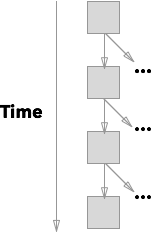
\includegraphics[width=4cm]{tree.png}
	\end{center}
	\caption{\textit{The traversal tree for the Alpha-Beta algorithm. Each decision is modeled as a box, which each arrow leading to another decision. Ellipses signify subtrees, which are effectively more trees following. The game decisions can be modeled through traversing down this tree as time passes. }}
	\label{fig:combatTree}
\end{figure}
\begin{figure}
	\begin{algorithmic}
	\Function{alphaBeta}{$s, d, m_0, \alpha, \beta$}
	\If {computationTime.elapsed}
	    \Call{timeout}{}
	\ElsIf
	    \If {terminal($s, d$)}
	        \Call{eval}{$s$}
	    \EndIf
	\EndIf
	
	\State toMove $\gets$ $s$.\Call{playerToMove}{policy}
	
	\While{\State $m$ $\gets$ s.\Call{nextMove}{toMove} }
		\If {$s$.bothCanMove and $m_0 = \theta$ and $d \neq$}
			\State $val$ $\gets$ \Call{alphaBeta}{$s, d-1, m, \alpha, \beta$}
		\Else
			\State $s'$ $\gets$ \Call{copy}{$s$}
			\If{$m_0 \neq \theta$}
				\State $s'$.\Call{doMove}{$m_0$}
			\EndIf
			\State $s'$.\Call{doMove}{$m_0$}
			\State $v$ $\gets$ \Call{alphaBeta}{$s', d-1, \theta, \alpha, \beta$}
		\EndIf
		\If{toMove = Branch and $v > \alpha$} 
			\State $\alpha$ $\gets$ $v$
		\EndIf
	\EndWhile
	\Return toMove = Branch ? $\alpha$ : $\beta$
	\EndFunction

	\end{algorithmic}
	\caption{The Alpha-Beta algorithm}
	\label{fig:alpha-beta}
\end{figure}
The Ultralisk AI employs an Alpha-Beta combat algorithm adapted from Churchill et al. (2012), which is, in essence, and fast search algorithm. If we consider the game state as each time period passes, each time period can consist of a tree, having branches at each potential decision, as shown in figure \ref{fig:combatTree}. The problem is then reduced into effectively an abstract tree traversal problem, which can be solved through the Alpha-Beta combat algorithm, shown in figure \ref{fig:alpha-beta}.

Given a player $p$ in state $s$, the next time $p$ is able to make a branching move is given by $\tau(s)$, where $\tau$ is the evaluation function for the next branch. 

We can then evaluate the sequential states with the $terminal(s, d)$ function, which decides when the call the evaluation function, parameterized by the maximal depth $d$, which is a track of how many nodes has already been traversed. $m_0$ is used to handle the \textit{delayed action effect}, which is when multiple decisions come up at a single period of time. $m_0$ holds the dummy value $\theta$ if only one decision needs to be made, but holds the secondary decision value if two more more decisions need to be made simultaneously. This way, we can pass in $m_0$ into the Alpha-Beta algorithm recursively until all simultaneous decisions are completed. \textit{Branch} is a branch function to modulate the outcome, which simply runs the neural network over the given parameters. 

\section{Results}
\begin{figure*}
	\begin{center}
		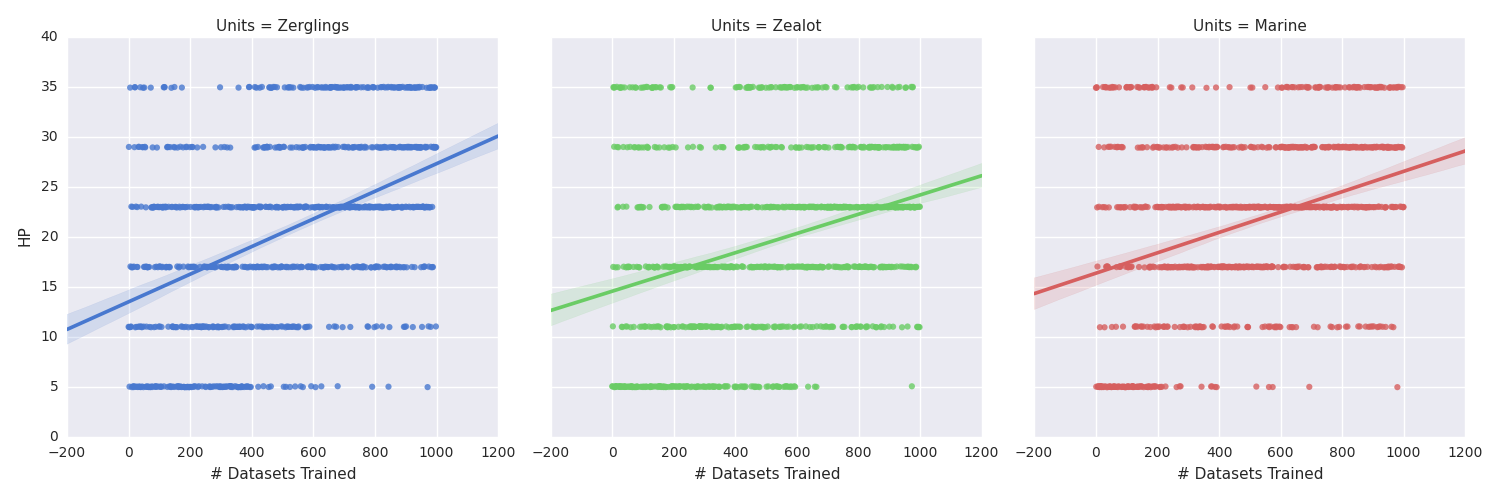
\includegraphics[width = \textwidth]{../plots/zerglingHP.png}
	\end{center}
	\caption{\textit{Results of the Starcraft combat. 1000 games were played against each of the three races, which results in the learning of the network. The X axis is the number of data samples the network has been trained on before, and the Y axis is the lowest remaining Zergling HP.}}
	\label{fig:results}
\end{figure*}
As shown in figure \ref{fig:results}, the number of data samples trained has a very large effect on the successfulness of the bot. The plots are the results of the Ultralisk AI battling against the three races, with the enemy deploying 3 Zerglings, 2 Zealots, and 3 Marines. Each data point has a X value of the number of datasets trained and a Y value of the lowest remaining Zergling HP. The lowest remaining Zergling HP is calculated by checking to see what the final unit(s) alive are, and then finding the HP value of the Zergling with the lowest HP. This data is collected through Starcraft itself, which is done by forcing the opponent computer to only build Zerglings/Zealots/Marines. 

As can be seen, the Ultralisk AI became very adept at deploying Zerglings in an optimal position against Marines and other Zerglings, but did not do as well against Zealots. This is due to the swarming nature of the Zerglings, the Ultralisk AI realized that Zerglings are more effective when they can fully surround an enemy, thus allowing all 3 to attack the same target at the same time. Because units continue to deal damage until they die, by focusing on a single target with the Zerglings, the enemy units can be dispatched in a quick manner. The reason why the Zerglings could not effectively attack Zealots was due to the high HP value of the Zerglings, the Zerglings simply could not focus attack down the Zealots before the Zealots killed the Zerglings. 
\section{Conclusions}
In this paper we have presented a small portion of Starcraft AI, which focuses solely on combat optimization on a small scale. If army sizes increase to beyond 10 units, the neural network had a very hard time generalizing and converging, resulting very ineffective combat deployment. We found that it was possible to optimize small scale combat by deploying units in such a manner that they would converge onto one location, thus surrounding the enemy and focusing it down. The next steps in the research would be to find a neural network generalization that could account for more than three units, for both the enemy and the ally. 
\end{document}